\documentclass[11pt]{article}
\usepackage{amsfonts,amsthm,amsmath,amssymb, hyperref, dsfont, enumitem, bbm}
\usepackage{array}
\usepackage{epsfig}
\usepackage{fullpage}
\usepackage{color}
\usepackage{epigraph}
\renewcommand{\epigraphflush}{center}
\usepackage[framemethod=tikz]{mdframed}
\usepackage{titlesec}
\usepackage{ellipsis}
\usepackage{subcaption}
\usepackage[normalem]{ulem}
\usepackage{todonotes}



\titleformat{\chapter}[display]
  {\normalfont\bfseries}{}{0pt}{\Huge}

\newif\ifdetails % fill in details that are omitted in lecture handout version


\newcommand{\qn}[1]{\todo[inline, color=brown!30]{Quynh: #1}}

% \newtheorem{definition}{Definition}
% \newtheorem{example}{Example}
% \newtheorem{remark}{Remark}
% \newtheorem{theorem}{Theorem}
% \newtheorem{exercise}{Exercise}

\newcommand{\R}{\mathbb{R}} 
\newcommand{\x}{\mathbf{x}} 
\newcommand{\y}{\mathbf{y}} 
\newcommand{\bb}{\mathbf{b}} 
\newcommand{\id}{\mathbbm{1}} 

\detailstrue %Change to detailsfalse when removing text

\begin{document}

%% Courtesy: Daniel Spielman, via Madhu Sudan --> Chi-Ning Chou --> Anurag Anshu

\theoremstyle{plain}
\newtheorem{theorem}{Theorem}[section]
\newtheorem{lemma}[theorem]{Lemma}
\newtheorem{example}[theorem]{Example}
\newtheorem{corollary}[theorem]{Corollary}
\theoremstyle{definition}
\newtheorem{definition}[theorem]{Definition}
\newtheorem*{mydefinition}{Definition}
\newtheorem{claim}[theorem]{Claim}
\newtheorem{fact}[theorem]{Fact}
\newtheorem{remark}[theorem]{Remark}
\newtheorem{exercise}[theorem]{Exercise}

%Left and right brackets
\newcommand {\br} [1] {\ensuremath{ \left( #1 \right) }}
\newcommand {\Br} [1] {\ensuremath{ \left[ #1 \right] }}


%Quantum notations
\newcommand {\norm}[1]{{\| #1 \|}}  
\newcommand {\bra} [1] {\ensuremath{ \left\langle #1 \right| }}
\newcommand {\ket} [1] {\ensuremath{ \left| #1 \right\rangle }}
\newcommand {\ketbratwo} [2] {\ensuremath{ \left| #1 \middle\rangle \middle\langle #2 \right| }}
\newcommand {\ketbra} [1] {\ketbratwo{#1}{#1}}
\newcommand{\braket}[2]{\langle#1|#2\rangle}
\newcommand{\Tr}[1]{\mathrm{Tr}\left(#1\right)}
\newcommand{\tr}[2]{\mathrm{Tr}_{#1}\left(#2\right)}
\newcommand{\PE}{\mathrm{PE}}
\newcommand{\EPR}{\mathrm{EPR}}
\newcommand{\CNOT}{\mathrm{CNOT}}
\newcommand{\CZ}{\mathrm{CZ}}

%Generic math symbols
\newcommand {\eps} {\varepsilon}
\newcommand{\tO}{\tilde{O}}
\newcommand{\ind}[1]{\mathrm{Ind}\left(#1\right)}
\newcommand {\id}{\mathds{1}}
\newcommand{\bitn}[1]{\ensuremath{\{0,1\}^{#1}}}
\newcommand{\bitone}{\ensuremath{\{0,1\}}}
\newcommand{\swp}{\mathrm{\textbf{Swap}}}

% Information theory and CS symbols
\newcommand {\prob} {\ensuremath{\mathrm{Prob}}}
\newcommand{\bigo}[1]{\mathcal{O}\left(#1\right)}
\newcommand{\omeg}[1]{\Omega\left(#1\right)}
\newcommand{\expec}{\mathbb{E}}
\newcommand{\relent}[2]{\mathrm{D}\left(#1\|#2\right)}
\newcommand{\KL}[2]{\mathrm{D}_{KL}\left(#1\|#2\right)}
\newcommand{\mutinf}[2]{\mathrm{I}\left(#1:#2\right)}
\newcommand{\condmutinf}[3]{\mathrm{I}\left(#1:#2|#3\right)}
\newcommand{\condent}[2]{\mathrm{S}\left(#1|#2\right)}
\newcommand{\ent}[1]{\mathrm{S}\left(#1\right)}
\newcommand{\cla}{\text{classical}}
\newcommand{\qua}{\text{quantum}}
\newcommand{\sym}{\textsf{sym}}

%Statistical measures
\newcommand{\F}{\mathrm{F}}
\newcommand{\tv}{\mathrm{TV}}
\newcommand{\Hol}{\mathrm{Hol}}
\newcommand{\hel}{\mathrm{Hd}}
\newcommand{\pur}{\mathrm{Pur}}
\newcommand{\scs}{\mathrm{succ}}
\newcommand{\err}{\mathrm{err}}
\newcommand{\can}{\mathrm{can}}
\newcommand{\Var}{\mathrm{Var}}

%Fancy alphabets
\def\cA{\mathcal{A}}
\def\cB{\mathcal{B}}
\def\cC{\mathcal{C}}
\def\cD{\mathcal{D}}
\def\cE{\mathcal{E}}
\def\cF{\mathcal{F}}
\def\cG{\mathcal{G}}
\def\cH{\mathcal{H}}
\def\cL{\mathcal{L}}
\def\cM{\mathcal{M}}
\def\cO{\mathcal{O}}
\def\cP{\mathcal{P}}
\def\cR{\mathcal{R}}
\def\cS{\mathcal{S}}
\def\cT{\mathcal{T}}
\def\cX{\mathcal{X}}
\def\N{\mathbb{N}}
\def\Z{\mathbb{Z}}



%%%%%%%%%%%%%%%%%%%%%%%%%%%%%%%%%%%%%%%%%%%%% 
%Commands below can be ignored by the students  
%%%%%%%%%%%%%%%%%%%%%%%%%%%%%%%%%%%%%%%%%%%%%
% Header
\newcommand{\handout}[5]{
   \renewcommand{\thepage}{#1-\arabic{page}}
   \noindent
   \begin{center}
   \framebox{
      \vbox{
    \hbox to 6.3in { {\bf #1}
     	 \hfill {\it #3} }
       \vspace{4mm}
       \hbox to 6.3in { {\Large \hfill #5  \hfill} }
       \vspace{2mm}
       \hbox to 6.3in { {\it #2 \hfill #4} }
      }
   }
   \end{center}
   \vspace*{4mm}
}

\newcommand{\lecture}[4]{\handout{#1}{#2}{Lecturer:
#3}{Scribe: #4}{Lecture #1}}



%Editing commands
\newcommand{\edit}[2]{\st{#1}\hspace{0.05in}\textcolor{blue}{#2}}
\newcommand{\suppress}[1]{}

\newcommand{\anote}[1]{{\color{red} \textbf{Anurag's note:} #1}}
\newcommand{\qnote}[1]{{\color{red} \textbf{Quynh's note:} #1}}
\newcommand{\hkn}[1]{{\color{orange} \textbf{Nguyen nu:} #1}}


%Itemizing and Equation shorthands
\newcommand{\beit}{\begin{itemize}}
\newcommand{\enit}{\end{itemize}}
\newcommand{\been}{\begin{enumerate}}
\newcommand{\enen}{\end{enumerate}}
\newcommand{\beq}{\begin{equation}}
\newcommand{\enq}{\end{equation}}
\newcommand{\beqst}{\begin{equation*}}
\newcommand{\enqst}{\end{equation*}}
\newcommand{\beqar}{\begin{eqnarray}}
\newcommand{\enqar}{\end{eqnarray}}
\newcommand{\beqarst}{\begin{eqnarray*}}
\newcommand{\enqarst}{\end{eqnarray*}}




\handout{SEAS 2025}{{\bf July ..., 2025}}{Instructor: }{TA: }{Lecture 4: Eigendecomposition part 2}


In charge: Nguyen name

\section{Eigenvalues and Eigenvectors: The Matrix's "Special" Directions}

When we multiply a vector $\x$ by a square matrix $A$, the resulting vector $A\x$ usually points in a different direction and might have a different length compared to $\x$.


However, for most square matrices, there are some special non-zero vectors $\x$ for which multiplying by $A$ only \textit{scales} the vector – it doesn't change its direction (except possibly flipping it $180^\circ$).

\begin{figure}[h]
\begin{center}
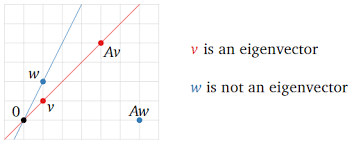
\includegraphics[width=0.6\textwidth]{LA Lecture notes/figures/lec3_eigenvector.png}
\end{center}
\caption{Action of matrix on eigenvector and general vector}
\end{figure}

These special vectors are called \textbf{eigenvectors}, and the scaling factors are called \textbf{eigenvalues}.

\begin{definition}[Eigenvalue and Eigenvector]
Let $A$ be an $n \times n$ square matrix. A non-zero vector $\x \in \R^n$ is called an \textbf{eigenvector} of $A$ if there exists a scalar $\lambda$ (lambda) such that
\begin{align} \label{eq:eigen_def}
    A\x = \lambda \x
\end{align}
The scalar $\lambda$ is called the \textbf{eigenvalue} corresponding to the eigenvector $\x$.
\end{definition}

\begin{remark}
\begin{itemize}
    \item Eigenvectors must be non-zero (the zero vector always satisfies $A\mathbf{0} = \lambda \mathbf{0}$, so it's not interesting).
    \item Eigenvalues $\lambda$ can be zero.
    \item Eigenvalues and eigenvectors can be complex numbers even if the matrix $A$ has only real entries, but we'll mostly focus on real ones here.
    \item If $\x$ is an eigenvector for eigenvalue $\lambda$, then any non-zero scalar multiple $c\x$ is also an eigenvector for the same eigenvalue $\lambda$, because $A(c\x) = c(A\x) = c(\lambda\x) = \lambda(c\x)$. Eigenvectors define special \textit{directions} or \textit{lines} through the origin.
\end{itemize}
\end{remark}

Think of eigenvectors as the "axes" along which the transformation represented by $A$ acts purely as a stretching or shrinking (or flipping if $\lambda < 0$).

\subsection{Finding Eigenvalues and Eigenvectors}

How do we find these special $\lambda$'s and $\x$'s for a given matrix $A$?
Let's rewrite the defining equation \eqref{eq:eigen_def}:
\begin{align*}
    A\x &= \lambda \x \\
    A\x - \lambda \x &= \mathbf{0} \\
    A\x - \lambda \id \x &= \mathbf{0} && \text{(Multiply } \lambda \x \text{ by } \id \text{)} \\
    (A - \lambda \id) \x &= \mathbf{0} && \text{(Factor out } \x \text{)}
\end{align*}
This equation $(A - \lambda \id) \x = \mathbf{0}$ is a \textit{homogeneous system of linear equations}. We are looking for non-zero solutions $\x$.
Remember from our theorem about invertibility: a homogeneous system $M\x = \mathbf{0}$ has non-zero solutions if and only if the matrix $M$ is \textbf{singular} (not invertible).

In our case, $M = (A - \lambda \id)$. So, we need the matrix $(A - \lambda \id)$ to be singular for a non-zero eigenvector $\x$ to exist.
And how do we test if a matrix is singular? Its determinant must be zero!

\begin{center}
\textit{We need: } $\det(A - \lambda \id) = 0$
\end{center}

This equation is called the \textbf{characteristic equation} of the matrix $A$.

Let's look at steps to find eigenvalues and eigenvectors:
\begin{enumerate}
    \item Form the characteristic equation: Calculate $\det(A - \lambda \id) = 0$. This will be a polynomial equation in $\lambda$.
    For $A = \begin{bmatrix} a & b \\ c & d \end{bmatrix}$, this is $\det \left( \begin{bmatrix} a & b \\ c & d \end{bmatrix} - \lambda \begin{bmatrix} 1 & 0 \\ 0 & 1 \end{bmatrix} \right) = \det \begin{bmatrix} a-\lambda & b \\ c & d-\lambda \end{bmatrix} = (a-\lambda)(d-\lambda) - bc = 0$.
    \item Solve for eigenvalues ($\lambda$): Find the roots of the characteristic polynomial. These roots are the eigenvalues of $A$.
    \item Find eigenvectors ($\x$) for each eigenvalue: For each eigenvalue $\lambda$ found in step 2, plug it back into the equation $(A - \lambda \id) \x = \mathbf{0}$ and solve this system for $\x$. The non-zero solutions are the eigenvectors corresponding to that $\lambda$. (Usually using Gauss-Jordan elimination on the augmented matrix $[A-\lambda \id \mid \mathbf{0}]$).
\end{enumerate}


\begin{example}
Find the eigenvalues and eigenvectors of $A = \begin{bmatrix} 3 & 1 \\ 1 & 3 \end{bmatrix}$.

\begin{enumerate}
    \item Characteristic Equation:
    \begin{align*} \det(A - \lambda \id) &= \det \begin{bmatrix} 3-\lambda & 1 \\ 1 & 3-\lambda \end{bmatrix} \\ &= (3-\lambda)(3-\lambda) - (1)(1) \\ &= (9 - 6\lambda + \lambda^2) - 1 \\ &= \lambda^2 - 6\lambda + 8 = 0 \end{align*}
    \item Solve for $\lambda$: Factor the polynomial: $(\lambda - 4)(\lambda - 2) = 0$. The eigenvalues are $\lambda_1 = 4$ and $\lambda_2 = 2$.
    \item Find eigenvectors:
    For $\lambda_1 = 4$: Solve $(A - 4\id)\x = \mathbf{0}$.
        \[ A - 4\id = \begin{bmatrix} 3-4 & 1 \\ 1 & 3-4 \end{bmatrix} = \begin{bmatrix} -1 & 1 \\ 1 & -1 \end{bmatrix} \]
        The system is $\begin{bmatrix} -1 & 1 \\ 1 & -1 \end{bmatrix} \begin{bmatrix} x_1 \\ x_2 \end{bmatrix} = \begin{bmatrix} 0 \\ 0 \end{bmatrix}$, which gives the equation $-x_1 + x_2 = 0$ (the second equation is just a multiple of the first). This means $x_1 = x_2$.
        Any vector where the components are equal (and not zero) is an eigenvector. Let's choose a simple one: $\x_1 = \begin{bmatrix} 1 \\ 1 \end{bmatrix}$.
        (Check: $A\x_1 = \begin{bmatrix} 3 & 1 \\ 1 & 3 \end{bmatrix} \begin{bmatrix} 1 \\ 1 \end{bmatrix} = \begin{bmatrix} 4 \\ 4 \end{bmatrix} = 4 \begin{bmatrix} 1 \\ 1 \end{bmatrix} = \lambda_1 \x_1$. Correct!)

        For $\lambda_2 = 2$: Solve $(A - 2\id)\x = \mathbf{0}$.
        \[ A - 2\id = \begin{bmatrix} 3-2 & 1 \\ 1 & 3-2 \end{bmatrix} = \begin{bmatrix} 1 & 1 \\ 1 & 1 \end{bmatrix} \]
        The system is $\begin{bmatrix} 1 & 1 \\ 1 & 1 \end{bmatrix} \begin{bmatrix} x_1 \\ x_2 \end{bmatrix} = \begin{bmatrix} 0 \\ 0 \end{bmatrix}$, which gives the equation $x_1 + x_2 = 0$. This means $x_1 = -x_2$.
        Any vector where the components are opposite (and not zero) is an eigenvector. Let's choose a simple one: $\x_2 = \begin{bmatrix} 1 \\ -1 \end{bmatrix}$.
        (Check: $A\x_2 = \begin{bmatrix} 3 & 1 \\ 1 & 3 \end{bmatrix} \begin{bmatrix} 1 \\ -1 \end{bmatrix} = \begin{bmatrix} 2 \\ -2 \end{bmatrix} = 2 \begin{bmatrix} 1 \\ -1 \end{bmatrix} = \lambda_2 \x_2$. Correct!)
\end{enumerate}
So, the eigenvalues are 4 and 2, with corresponding eigenvectors (examples) $\begin{bmatrix} 1 \\ 1 \end{bmatrix}$ and $\begin{bmatrix} 1 \\ -1 \end{bmatrix}$.
\end{example}

\section{Eigendecomposition: Understanding Matrices Better}

Eigenvalues and eigenvectors help us understand the "essence" of a matrix transformation. If a matrix $A$ (size $n \times n$) has enough linearly independent eigenvectors to form a basis for $\R^n$ (this happens if it has $n$ distinct eigenvalues, or in some other cases like symmetric matrices), we can do something called \textbf{eigendecomposition}.

Think about it: if we use the eigenvectors as our coordinate system axes, the transformation $A$ becomes much simpler – it just stretches or shrinks along these axes by the eigenvalue amounts!

\begin{theorem}[Eigendecomposition]
Let $A$ be an $n \times n$ matrix. If $A$ has $n$ linearly independent eigenvectors $\x_1, \x_2, \ldots, \x_n$ corresponding to eigenvalues $\lambda_1, \lambda_2, \ldots, \lambda_n$ (which may not be distinct), then $A$ can be factored as:
\begin{align} \label{eq:eigendecomp}
    A = P D P^{-1}
\end{align}
where:
\begin{itemize}
    \item $P$ is an invertible matrix whose columns are the eigenvectors of $A$:
    \[ P = [\x_1 \mid \x_2 \mid \cdots \mid \x_n] \]
    \item $D$ is a diagonal matrix whose diagonal entries are the corresponding eigenvalues:
    \[ D = \text{diag}(\lambda_1, \lambda_2, \dots \lambda_n) := \begin{bmatrix}
        \lambda_1 & 0 & \cdots & 0 \\
        0 & \lambda_2 & \cdots & 0 \\
        \vdots & \vdots & \ddots & \vdots \\
        0 & 0 & \cdots & \lambda_n
    \end{bmatrix} \]
\end{itemize}
This is called the \textbf{eigendecomposition} or \textbf{spectral decomposition} of $A$. A matrix that can be decomposed in this way is called \textbf{diagonalizable}.
\end{theorem}

So what does $A = PDP^{-1}$ mean intuitively? Applying $A$ to a vector $\mathbf{v}$ (i.e., calculating $A\mathbf{v}$) can be thought of in three steps:
\begin{enumerate}
    \item $P^{-1}\mathbf{v}$: Change coordinates from the standard basis to the eigenvector basis. Find out "how much" of $\mathbf{v}$ lies along each eigenvector direction.
    \item $D(P^{-1}\mathbf{v})$: In the eigenvector basis, the transformation is simple! Just scale each component (along the eigenvector axes) by the corresponding eigenvalue $\lambda_i$. This is easy because $D$ is diagonal.
    \item $P(D P^{-1}\mathbf{v})$: Change the coordinates of the scaled result back from the eigenvector basis to the standard basis.
\end{enumerate}
So, eigendecomposition tells us that the complex action of $A$ can be broken down into: change basis, simple scaling, change basis back.

\begin{example}
For our matrix $A = \begin{bmatrix} 3 & 1 \\ 1 & 3 \end{bmatrix}$ with $\lambda_1=4, \x_1=\begin{bmatrix} 1 \\ 1 \end{bmatrix}$ and $\lambda_2=2, \x_2=\begin{bmatrix} 1 \\ -1 \end{bmatrix}$.
We have:
\[ P = \begin{bmatrix} 1 & 1 \\ 1 & -1 \end{bmatrix}, \quad D = \begin{bmatrix} 4 & 0 \\ 0 & 2 \end{bmatrix} \]
We need $P^{-1}$. Using the formula for 2x2 inverse ($P^{-1} = \frac{1}{ad-bc} \begin{bmatrix} d & -b \\ -c & a \end{bmatrix}$):
\[ \det(P) = (1)(-1) - (1)(1) = -2 \]
\[ P^{-1} = \frac{1}{-2} \begin{bmatrix} -1 & -1 \\ -1 & 1 \end{bmatrix} = \begin{bmatrix} 1/2 & 1/2 \\ 1/2 & -1/2 \end{bmatrix} \]
Let's check the decomposition: $A = PDP^{-1}$?
\begin{align*} PDP^{-1} &= \begin{bmatrix} 1 & 1 \\ 1 & -1 \end{bmatrix} \begin{bmatrix} 4 & 0 \\ 0 & 2 \end{bmatrix} \begin{bmatrix} 1/2 & 1/2 \\ 1/2 & -1/2 \end{bmatrix} \\ &= \begin{bmatrix} 1 & 1 \\ 1 & -1 \end{bmatrix} \left( \begin{bmatrix} 4 & 0 \\ 0 & 2 \end{bmatrix} \begin{bmatrix} 1/2 & 1/2 \\ 1/2 & -1/2 \end{bmatrix} \right) \\ &= \begin{bmatrix} 1 & 1 \\ 1 & -1 \end{bmatrix} \begin{bmatrix} (4)(1/2) + (0)(1/2) & (4)(1/2) + (0)(-1/2) \\ (0)(1/2) + (2)(1/2) & (0)(1/2) + (2)(-1/2) \end{bmatrix} \\ &= \begin{bmatrix} 1 & 1 \\ 1 & -1 \end{bmatrix} \begin{bmatrix} 2 & 2 \\ 1 & -1 \end{bmatrix} \\ &= \begin{bmatrix} (1)(2)+(1)(1) & (1)(2)+(1)(-1) \\ (1)(2)+(-1)(1) & (1)(2)+(-1)(-1) \end{bmatrix} \\ &= \begin{bmatrix} 3 & 1 \\ 1 & 3 \end{bmatrix} \end{align*}
It works! $A = PDP^{-1}$.

\end{example}

\begin{remark}
\begin{itemize}
    \item Not all matrices are diagonalizable (meaning they don't have enough linearly independent eigenvectors). We will learn about a generalization of eigendecomposition that works for any matrix in the next lecture.
    \item Eigendecomposition is very powerful. For example, calculating powers of $A$ becomes easy: $A^k = (PDP^{-1})^k = P D P^{-1} P D P^{-1} \cdots P D P^{-1} = P D^k P^{-1}$. Calculating $D^k$ is trivial (just raise the diagonal elements to the power $k$). This has applications in areas like population modeling, Markov chains, and solving differential equations.
\end{itemize}
\end{remark}

\begin{exercise}
    Prove the norm-preserving property of orthogonal matrices using eigendecomposition.
\end{exercise}

\begin{exercise}
    Given the eigendecomposition of a diagonalizable matrix $A$, 
    \begin{align*}
        A = PDP^{-1}
    \end{align*}
    where $D = \text{diag}(\lambda_1, \lambda_2, \dots \lambda_n)$.
    Find the expression for $A^{-1}$.
\end{exercise}

\section{Singlular Value Decomposition (SVD): A decomposition that works every time}
We saw that eigendecomposition ($A = PDP^{-1}$) is super useful for understanding square matrices $A$. It tells us the special "axes" (eigenvectors) along which the matrix $A$ simply acts by stretching or shrinking (by the eigenvalues).

But eigendecomposition has crucial limitations. Firstly, it only works for \textit{square} matrices. Besides, not all square matrices have enough linearly independent eigenvectors to be decomposed this way (i.e., not all are diagonalizable).

Luckily, there's a more powerful tool called the \textbf{Singular Value Decomposition (SVD)} that works for \textit{any} matrix, whether it's square or rectangular!

In the same spirit of eigendecomposition, SVD breaks down any matrix $A$ into the product of three simpler matrices. Recall that eigendecomposition tells us the complex action of $A$ can be broken down into: change basis (a rotation), simple scaling, change basis back (another rotation). Similarly, SVD tells us that any linear transformation (represented by matrix $A$) can be thought of as a combination of:
a rotation in the input space followed by a scaling along principal axes, and then a rotation in the output space. 

\begin{theorem}[Singular Value Decomposition - SVD]
For any matrix $A$ of size $m \times n$. There exist matrices $U$, $\Sigma$ (capital Sigma), and $V$ such that:
\begin{align} \label{eq:svd}
    A = U \Sigma V^T
\end{align}
where:
\begin{itemize}
    \item $U$ is an $m \times m$ \textbf{orthogonal} matrix. (Its columns are the \textbf{left singular vectors}, which are orthonormal. $U^T U = U U^T = \id_m$). It represents the rotation in the output space ($m$-dimensional space).
    \item $\Sigma$ is an $m \times n$ "diagonal-like" matrix. Its entries on the main diagonal are the \textbf{singular values} $\sigma_1, \sigma_2, \ldots, \sigma_r$ (where $r$ is the rank of matrix $A$). These singular values are always non-negative and represent how much the matrix $A$ stretches or shrinks space along its principal directions. All other entries in $\Sigma$ are zero. It represents the scaling part.
    \[
    \Sigma = \begin{bmatrix}
        \sigma_1 & 0 & \cdots & 0 & \cdots & 0 \\
        0 & \sigma_2 & \cdots & 0 & \cdots & 0 \\
        \vdots & \vdots & \ddots & \vdots & & \vdots \\
        0 & 0 & \cdots & \sigma_r & \cdots & 0 \\
        \vdots & \vdots & & \vdots & \ddots & \vdots \\
        0 & 0 & \cdots & 0 & \cdots & 0
    \end{bmatrix}
    \quad \text{(Example structure for } m \ge n \text{)}
    \]
    \item $V$ is an $n \times n$ \textbf{orthogonal} matrix. (Its columns are the \textbf{right singular vectors}, which are orthonormal. $V^T V = V V^T = \id_n$). $V^T$ represents the rotation in the input space ($n$-dimensional space).
\end{itemize}
\end{theorem}
Singular values connect to eigenvalues through the following result (prove it!). This shows SVD is deeply related to eigendecomposition.
\begin{theorem}
    The squares of the singular values ($\sigma_i^2$) are the eigenvalues of the square matrices $A^T A$ and $AA^T$. The columns of $V$ are the eigenvectors of $A^T A$, and the columns of $U$ are the eigenvectors of $AA^T$.
\end{theorem}

Ok, being able to decompose an arbitrary matrix is cool, but why should we care? I'm glad you asked! One major application of SVD is finding the best way to approximate a matrix $A$ with a simpler matrix of lower rank. If we take the SVD $A = U \Sigma V^T$ and keep only the largest $k$ singular values in $\Sigma$ (setting the rest to zero, let's call this $\Sigma_k$), then the matrix $A_k = U \Sigma_k V^T$ is the \textit{best} rank-$k$ approximation of $A$. This is the result known as the low-rank approximation theorem or, if you prefer names, Eckart–Young–Mirsky theorem.

This is a very useful result. Think about image compression: An image can be represented as a matrix of pixel values. If we compute the SVD of this matrix, we often find that many singular values are very small. By keeping only the largest $k$ singular values (and the corresponding vectors in $U$ and $V$), we can reconstruct an approximate image $A_k$ that looks very similar to the original but requires much less data to store ($k$ singular values + parts of $U$ and $V$ instead of the whole matrix $A$).

\section{Measuring the Size of Matrices: Matrix Norms}
We know how to measure the length (or magnitude) of a vector using norms, like the familiar Euclidean norm $\|v\|_2 = \sqrt{\sum_i v_i^2}$. But how do we measure the "size" or "magnitude" of a whole matrix? Matrix norms do exactly this. 
There are many different matrix norms, but we'll focus on two important families.

\subsection{The Frobenius Norm}
This is probably the most intuitive matrix norm. It's directly analogous to the Euclidean norm for vectors. You just treat the matrix elements as if they were entries in one long vector. In other words, it is nothing more than the Euclidean norm of the vectorization of A!

\begin{definition}[Frobenius norm]
    For an $m \times n$ matrix $A$, the Frobenius norm, denoted $\|A\|_F$, is defined as:
\[
\|A\|_F = \sqrt{\sum_{i=1}^m \sum_{j=1}^n |A_{ij}|^2}
\]
\end{definition} 
It's the square root of the sum of the squares of all the elements in the matrix.

\begin{example}
Let $A = \begin{bmatrix} 1 & -2 \\ 3 & 0 \end{bmatrix}$.
\[ \|A\|_F = \sqrt{1^2 + (-2)^2 + 3^2 + 0^2} = \sqrt{1 + 4 + 9 + 0} = \sqrt{14} \]
\end{example}

\subsection{Schatten Norms}
Schatten norms are a more general family defined using the \textbf{singular values} $\sigma_i$ obtained from SVD.

\begin{definition}[Schatten norm]
    The Schatten $p$-norm of a matrix $A$ (with singular values $\sigma_i$) is defined as the $L_p$ norm of the vector of its singular values:
\[
\|A\|_{S_p} = \left( \sum_i \sigma_i^p \right)^{1/p}
\]
\end{definition} 

\begin{example}
\begin{itemize}
    \item \textbf{$p=2$: Schatten-2 Norm.} This turns out to be exactly the Frobenius norm! $\|A\|_{S_2} = \left( \sum_i \sigma_i^2 \right)^{1/2}$ (see Exercise below).
    \item \textbf{$p=1$: Schatten-1 Norm (or Nuclear Norm).} $\|A\|_{*} = \|A\|_{S_1} = \sum_i \sigma_i$. This norm is important in machine learning and optimization, often used to encourage matrices to have low rank.
    \item \textbf{$p=\infty$: Schatten-$\infty$ Norm (or Spectral Norm).} $\|A\|_{S_\infty} = \max_i \sigma_i$. This norm measures the maximum stretching factor the matrix applies to any vector. It's equal to the largest singular value.
\end{itemize}
    
\end{example}
While different norms give different numerical values for the size of a matrix, they are all "equivalent" in a certain sense. This means that if one norm of a matrix is small, all other norms will also be relatively small, and if one norm is large, others will be large too. They all capture the general idea of matrix magnitude, just with different sensitivities. In particular, the Schatten $p-$norm and $q-$norm are related by
\begin{align*}
    \norm{A}_{S_q} \leq \norm{A}_{S_p} \leq n^{1/p-1/q}\norm{A}_{S_q}, \,  \forall 0<p<q
\end{align*}

But, as we shall see, although all norms are equal, some are more equal than others in specific application!

\begin{exercise}
Prove that the Schatten-2 norm is equal to the Frobenius norm ($\|A\|_{S_2} = \|A\|_F$).
\end{exercise}

\begin{exercise}
Prove that the Frobenius norm is equal to the standard Euclidean ($L_2$) norm of the vector formed by stacking all columns of the matrix $A$ into one long vector. This operation is called vectorization, denoted $\text{vec}(A)$. Show $\|A\|_F = \|\text{vec}(A)\|_2$.
\end{exercise}

% \begin{exercise}
% Prove that all Schatten norm are unitarily invariant
% \end{exercise}


% \section{Eigendecomposition}
% More exercises on eigen decomp,

% Visualization of matrix multiplication using eigendecomp (E.g Fig 2.3 in \href{https://www.deeplearningbook.org/contents/linear_algebra.html}{this book})


% \section{Matrix norms}
% \begin{itemize}
%     \item Schatten norms
%     \item Frobenius norm
% \end{itemize}

% Exercise: prove Schatten-2 norm is equal to Frobenius norm.

% Exercise: prove Frobenius norm is equal to ell-2 norm of vectorization

% \section{Positive semidefinite matrices}

% Motivate applications of psd matrices




% \qn{NOTE: Will we cover pseudoinverse? Probably in a later lecture or in the ML lecs.}



\end{document}